\documentclass{article}
\usepackage{aaai}
\usepackage{graphicx}
\usepackage[ruled, vlined, linesnumbered]{algorithm2e}
\usepackage[toc, page]{appendix}

% Big margins for now so people can take notes/scribbles.
%\usepackage{fullpage}

\title{Parallel Best NBlock First}
%\author{Ethan Burns \and Seth Lemons \and Wheeler Ruml \\
%  Department of Computer Science \\
%  University of New Hampshire \\
%  Durham, NH 03824 USA \\
%  \{eaburns,seth.lemons, ruml\}@unh.edu}
\author{Ethan Burns
  Department of Computer Science \\
  University of New Hampshire \\
  Durham, NH 03824 USA \\
  eaburns@unh.edu}
\date{\today}

\begin{document}
\maketitle

\begin{abstract}
  A lot of work in heuristic search focuses on solving larger and larger
  problems.  Various techniques have been developed for making heuristic
  search more memory efficient.  Other techniques have been developed
  that allow heuristic search to make use of external storage devices
  (such as hard disks) to increase their memory capacity.  In this paper
  we build on some of the techniques used for external memory search to
  create a parallel best-first style search to be used to more quickly
  solve smaller search domains.
\end{abstract}

\section{Introduction}

As microprocessor manufacturers build processors with more and more
cores, software developers are being pressured to create algorithms to
make better use of the newly available parallelism.  In the field of
artificial intelligence it is always necessary to solve problems more
quickly.  A trend in current research on heuristic search, however,
seems to be focusing on finding solutions in larger and larger search
domains instead of solving smaller domains faster.  For this work our
goal was to attempt to use parallelism to solve some problems that are
traditionally considered small more quickly.

In a typical (serial) best-first search algorithm, an \emph{open-list}
and \emph{closed-list} of nodes are maintained.  The open-list
contains nodes on the search frontier that have yet to be searched
(expanded).  The open-list is usually sorted on the f-value for each
node, where $f(n)$ for a node $n$ is the estimated cost for a solution
path which goes through $n$.  The closed-list contains all nodes
which have already been searched, and it is used to detect cycles in
the search graph.  The process of detection nodes that have already
been searched is called \emph{duplicate detection}.  In a serial
best-first search, a node is added to the closed-list the first time
that the search encounters it.  If a node is encountered again during
the search process, it is ignored since it has already been expanded.
This process breaks cycles and eliminates extra, wasted, search
effort.

One of the greatest challenges of parallel heuristic search is
reducing synchronization overhead.  This can be seen by looking at a
naive approach to parallelizing heuristic search where a global open
and closed list are used with a mutual exclusion lock (called a
\emph{mutex}).  The problem with this approach is that, as the number
of processors increases, there will be an increasing amount of
contention on these two data structures.  This will create a large
bottle-neck, greatly slowing down the search.

Various methods have been proposed to attempt to alleviate the
overhead of synchronizing the access to global data structures in
parallel heuristic search algorithms.  The problem with most of these
approaches is that they still require processors to lock a mutex
during the ``fast-path'' of the search -- while expanding nodes.
Other algorithms make use of depth-first or breadth-first search
instead of using a best-first ordering to reduce contention.  While
these methods may scale with more processors, they still suffer from
the brute-force nature of the depth-first and breadth-first search
methods.  Each of these techniques also suffers from additional
disadvantages: depth-first search performs \emph{very} poorly on
domains which have a lot of duplicates, and breadth-first search
performs poorly on domains which do not have unit cost edges.

The algorithm which is presented in this paper extends some ideas
which were developed for external memory search -- an area which
shares some of the same problems as parallel search.  Our algorithm,
which is called Parallel Best NBlock First (PBNF), allows processors
to acquire sections of a search space in a manor which allows for
periods of synchronization-free search.  Additionally, this method
lets the search to progress in a best-first manor which detects
duplicates and can perform well with non-uniform move costs.  Moreover
PBNF can be trivially adapted to use sub-optimal, weighted or
pessimistic heuristics.  We demonstrate the performance of our
algorithm on a handful of common search domains, including grid-world
and the sliding tiles domain.  Our results show that this algorithm
outperforms all previously proposed algorithms which we compare
against.

\section{Previous Work}

Before describing our new algorithm, we will discuss some of the
previous work in parallel-heuristic search.  In this section we also
describe some serial algorithms from which we gathered some of the
ideas for our new parallel approach.

\subsection{Parallel Retracting A*}

There has been a handful of algorithms created that attempt to
alleviate the amount of contention between processors by making use of
distributed open and closed lists instead of using global data
structures.  One such algorithm is Parallel Retracting A* (PRA*)
\cite{evett:pra}.  PRA* attempts to reduce synchronization in this
manor.  In PRA* a hashing scheme is used to divide the search nodes up
among all of the available processors.  Each time a processor expands
a node, passes the node to the appropriate processor dictated by the
hash function.  Each processor is then in charge of expanding and
detecting duplicates for all of the nodes that hash to it.  This
method allows duplicate detection to happen without communicating
between all of the processors, it also reduces the amount of
contention on the open-list by distributing it amongst all of the
processors.  The true PRA* algorithm also use a node-retraction scheme
to reduce the amount of memory that a search uses.  For this work, we
are only concerned with problems that fit into memory, and our
interest in PRA* is for its unique method of splitting the search
space amongst processors, not its node-retraction scheme.

One of the problems that PRA* encounters is that, while no
synchronization is required for duplicate detection, there is a
substantial amount of overhead incurred by the message passing that is
used to move nodes to their respective processors.  In a shared memory
system, each processor must have a synchronized queue which all of the
other processors have the ability to add search nodes to.  While this
is less of a bottle-neck than having a single global, shared
open-list, we have found that it is still very expensive.  We
demonstrate the performance for our implementation of PRA* later in
this paper and show that our new algorithm performs significantly
better.

\subsection{Structured Duplicate Detection}

Structured Duplicate Detection or SDD \cite{zhou:sdd} is a method for
performing external memory search.  SDD uses a projection function, a
many-to-one mapping from states in a search space to states in an
abstract space, to decompose a search graph.  The projection function
creates an abstract space of nodes that are projections, or images, of
the nodes in the original state space.  Since the projection function
is a many-to-one mapping, the abstract space is significantly smaller
than the original search space.  For a projection function $p$, $y$ is
said to be the \emph{image} of a node $x$ if $p(x) = y$.  Additionally
$y'$ is a successor of $y$, in the abstract graph, if there are two
states $x$ and $x'$ such that $x'$ is a successor of $x$, $y$ is the
image of $x$ and $y'$ is the image of $x'$.  In other words:

\begin{eqnarray*}
  &&x' \in successors(x) \wedge p(x) = y \wedge p(x') = y' \\
  &\Rightarrow& y' \in successors(y)
\end{eqnarray*}

In the description of the SDD algorithm, Zhou and Hansen use the term
\emph{nblock} to refer to all nodes in the original state space that
have the same image in the abstract space.  Throughout the remainder
of this paper, the terms ``abstract state'', and ``nblock'' will be
used interchangeably, as each nblock corresponds to a single abstract
state.

Zhou and Hansen show that, while performing duplicate detection, only
nodes which reside within the same nblock must be checked for
duplicates.  This is because, for a node $x$ which is a duplicate of a
node $z$, both $x$ and $z$ will project to the same abstract state
(and therefore reside in the same nblock) Intuitively, this makes
sense, because both $x$ and $z$ are the same node.  This leads to the
idea of a \emph{duplicate detection scope}.  By the definition of the
successor set of an abstract node: any child node $x'$ of a node $x$,
in the original state space, will have an image $p(x') \in
successors(p(x))$, and therefore when performing duplicate detection
for $x'$ the only nodes that must be checked are in the nblock $p(x')
\in successors(p(x))$.  For this reason, $successors(p(x))$ is called
the duplicate detection scope of the nblock $p(x)$ -- no other nodes
in the original state space will ever need to be consulted for
duplicate detection when expanding nodes in the nblock $p(x)$.

This idea can be shown using the sliding tile puzzle as an example.
One possible projection function for the sliding tiles puzzle would be
to only look at the position of the empty tile.  For example: all
states with the empty tile in the upper left-hand corner (position 0)
would map to the nblock shown on the left in Figure
\ref{fig:tile-abstraction}, where the grayed square represents the
position of the empty tile.  Using this abstraction, there are sixteen
possible abstract states, one for each possible position of the empty
tile.  It is easy to see that all of the children of a state in the
nblock shown on the left in Figure \ref{fig:tile-abstraction} will
have the empty tile in either position 1 or 4 (either by sliding the
tile in position 1 to the left, or by sliding the tile in position 4
up).  The image on the right, in Figure \ref{fig:tile-abstraction},
shows the duplicate detection scope for the nblock shown on the left
in this figure.  Any of the children of a state in the nblock shown on
the left in Figure \ref{fig:tile-abstraction} will fall into one of
the two nblocks shown on the right.

\begin{figure*}[t]
  \begin{center}
    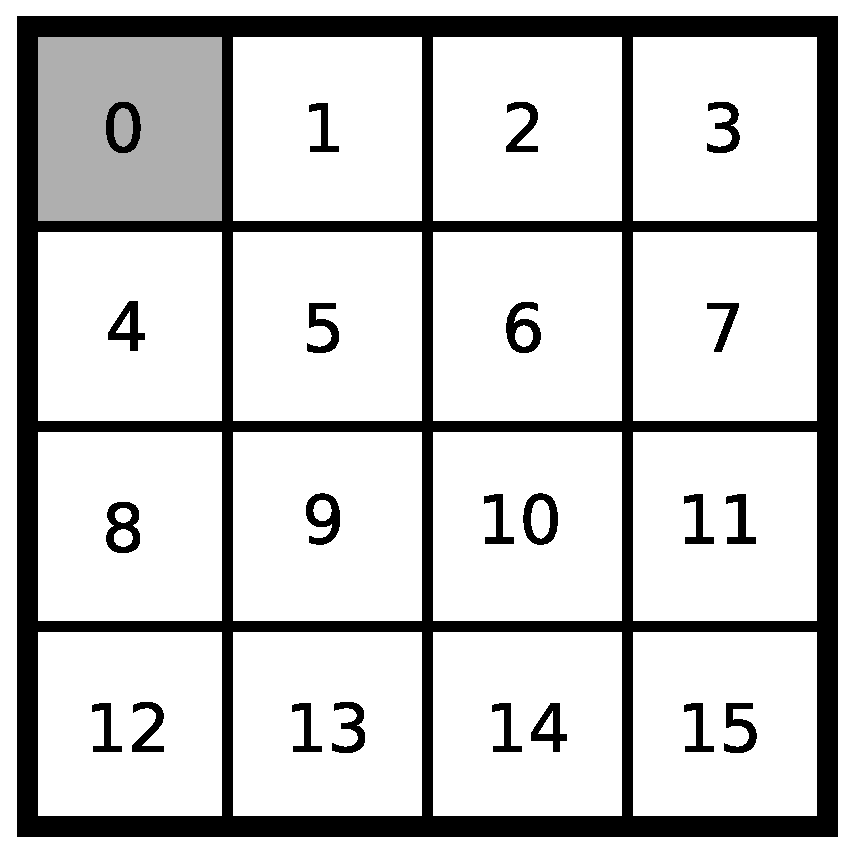
\includegraphics[width=1.5in]{images/tile-abstraction.eps}
    \hspace{4cm}
    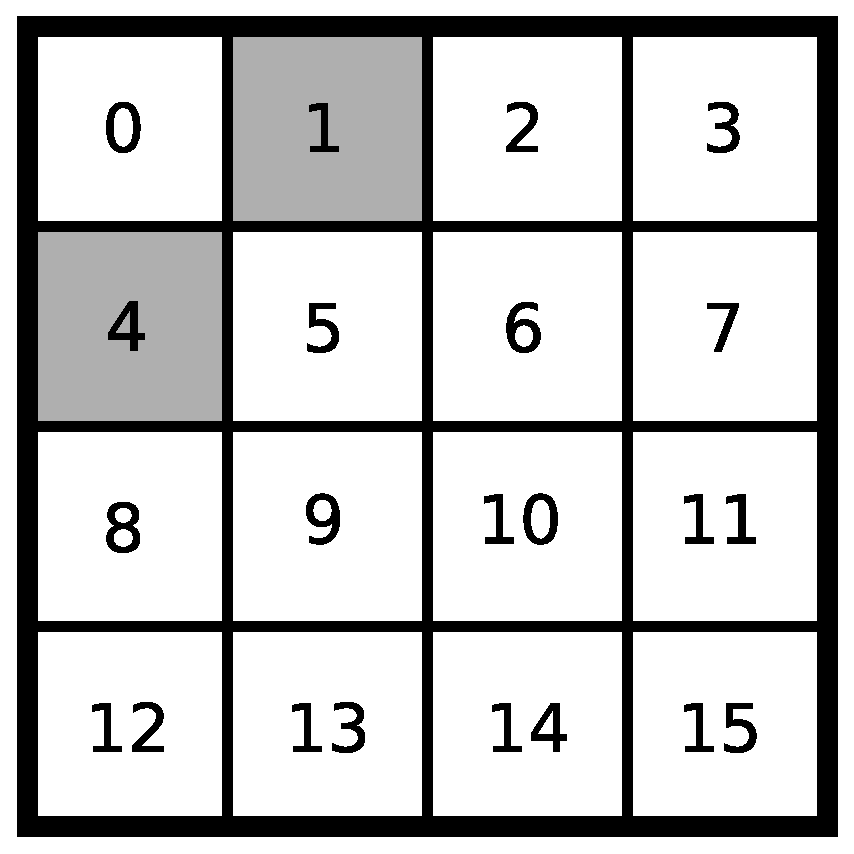
\includegraphics[width=1.5in]{images/duplicate-detection-scope.eps}
    \caption{The abstract image of all states with a empty tile in
      position 0 (left).  The duplicate detection scope of the
      abstract state with the empty tile in position 0 (left).}
    \label{fig:tile-abstraction}
  \end{center}
\end{figure*}

The main focus of the SDD approach is using state space decomposition
so that generated nodes can be explicitly moved to a secondary storage
device (such as a disk drive) when they are not in the duplicate
detection scope of the nblock being expanded and therefore are not
needed.  The SDD approach uses breadth-first heuristic search, where
only the nodes of the current search depth in a single nblock are
searched at a time.  Nodes of this nblock are expanded from the
current depth-layer and their children are placed into the next-depth
layer of their corresponding nblocks.  When the current nblock has no
more nodes at the current depth-layer, it is swapped for another
nblock which does have open nodes at this depth.  If no more nblocks
have nodes at the search depth, the search progresses to the next
layer (which contains the children nodes of the previous layer).  This
procedure repeats until a goal is found, or until no nodes
remain. Since duplicates can only fall into the duplicate detection
scope of the nblock being searched, the remainder of the nodes can be
pushed off to disk, instead of being stored in main-memory.  Nblocks
can then be intelligently swapped into and out of main-memory as the
search progresses.

\subsection{Parallel Structured Duplicate Detection (PSDD)}

While the motivation of SDD is to have explicit control over which
portions of a search space reside in main-memory.  Zhou and Hansen
also show that this approach lends itself to parallelization
\cite{zhou:psd}.  The parallel SDD (or PSDD) algorithm uses the graph
of nblocks to find \emph{disjoint duplicate detection scopes}, or
duplicate detection scopes that do not overlap.  Nblocks with disjoint
duplicate detection scopes can be searched in parallel without any
locking or contention.  In order to find nblocks with disjoint
duplicate detection scopes the concept of a \emph{free} nblock is
introduced.  An nblock $b$ is considered to be free if no processor
has acquired an nblock in $successors(b)$ -- in other words, if all
other processors are searching nblocks with duplicate detection scopes
which are disjoint from that of $b$.  Free nblocks are found by
tracking a $\sigma(b)$ value for each nblock $b$, where $\sigma(b)$ is
the number of nblocks in $successors(b)$ that are in use by another
processor.  Any nblock $b$ with $\sigma(b) = 0$ is free, and therefore
a processor can acquire $b$ and its duplicate detection scope for a
period of lock free expansion.  Besides tracking disjoint duplicate
detection scopes, the search procedure of PSDD is the same as that of
SDD; the search progresses by searching one depth-layer at a time
until a goal is found or the search space is exhausted.

PSDD is an attractive algorithm because it reduces the amount of
contention between processors by allowing for lock-free periods of
expansion.  The problem with the PSDD approach, however, is that it
performs a breadth-first style of search, and requires all of the
processors to synchronize between each layer.  Furthermore because of
the breadth-first nature of PSDD, the algorithm will not perform well
on domains which do not have unit-cost moves.  This is because, in
such a domain, each layer of the search may have only a small number
of new nodes.  If there are not enough nodes in a layer to amortize
the cost of synchronizing all of the processors between layers, or
worse if there are not enough nodes to keep all processors busy, then
the search will perform very poorly.

\subsubsection{Best-First PSDD}

Typically the PSDD algorithm uses breadth-first search because it can
be made more memory efficient than a typical best-first search
\cite{zhou:bhs}.  Since PSDD was created to solve very large problems,
memory efficiency is beneficial even with the use of external storage
(for example, I/O operations can be smaller and less frequent).  As
previously mentioned, however, this presents a problem with
non-unit-cost domains.  Zhou and Hansen anticipate this problem and
suggest modification to the SDD (and PSDD) algorithm to make it search
in a best-first order \cite{zhou:sdd} (we call this modified PSDD
algorithm BFPSDD for best-first PSDD).  This modification performs a
layer-by-layer search like SDD and PSDD but, in this case, each layer
consists of all of the nodes with the same f-value.  The BFPSDD
algorithm stores all nblocks in a heap which is sorted by the best
f-value of the best node in each nblock.  At each layer, BFPSDD
populates its list of free nblocks with all of the nblocks which have
the next best f-value.  When searching an nblocks, a processor
searches all of the nodes in the nblock which have an f-value equal to
the current layer's f-value.  Once all of the nodes with a given
f-value are searched, all of the processors synchronize and the search
progresses to the next f-value layer by re-populating the free list
with all nblocks from the heap-of-nblocks that have the next best
f-value.  It is easy to see that this search will progress in a
best-first manor and this means that it will not perform as poorly on
non-unit-cost domains.  In real-valued domains, however, this
algorithm may not perform well since, again, layers may contain only a
very small number of nodes with the same f-value.

%% mention how there is yet another possible extension to PSDD to make
%% it perform well on real-valued domains.

\subsection{Localizing A*}

An alternative approach to external memory search for improving
efficiency in large search spaces is to slightly loosen the node
ordering restriction of A* as is done by Edelkamp and Schrodl
\cite{edelkamp:loc}.  Edelkamp and Schrodl create an algorithm that
uses a looser node ordering than A* in order to achieve a better
memory locality. We refer to this algorithm as lA* (for localized A*).
While lA* expands more nodes than A* does, the intuition is that lA*
can achieve better performance than A* for large searches because it
can reduce the number of virtual-memory operations that swap to disk.

lA* uses a data structure called a \emph{heap-of-heaps} to order its
node expansions.  A heap-of-heaps, $H$, is composed of elements $H_0$,
$H_1$, ..., $H_n$, where each element $H_i$ is a heap of search nodes
that reside in the same page of memory.  The heap-of-heaps, $H$, is
loosely sorted based on the f-values of the best nodes of each heap
$H_i$ (denoted as $best(H_i)$).  The lA* procedure searches the best
heap $H_0$, of the heap-of-heaps, until $best(H_1) + \Delta >
best(H_0)$, where $H_1$ is the new best heap on $H$ after the removal
of $H_0$.  The $\Delta$ value allows the search to expand a set of
nodes in $H_0$ which may not have the best f-values, but that have
better memory locality with respect to the previously expanded nodes.

Since lA* prefers nodes with better memory locality, it reduces the
number of page-faults, and virtual memory swap operations that the
operating system must perform.  The tradeoff is that the first
solution found by lA* may be sub-optimal since it is not searching in
strict f-value order.  To fix this problem, lA* doesn't return its
first solution, instead it behaves like an any-time search algorithm
by continuing the search and pruning on the f-value of incumbent
solutions.  Since the f-value of an incumbent solution is an
upper-bound on the optimal solution, the search can stop when there
are no frontier nodes that have f-values less than the current
incumbent -- this means that the current incumbent solution \emph{is}
the optimal solution.

\section{Parallel Best NBlock First (PBNF)}

In order to get the benefits of lock-free expansion and duplicate
detection, which are provided by the PSDD algorithm, without the need
for layer-synchronization, we have created an algorithm that combines
the ideas from PSDD and lA* which we call Parallel Best NBlock First
(PBNF).  The PBNF algorithm maintains a heap of free nblocks where
each nblock has a heap of open nodes sorted on f-value and a hash
table of closed nodes which have already been searched.  Processors
use the heap of free nblocks to attempt to acquire the free nblock
with the best open node.  A processor will search its acquired nblock
as long as it contains nodes which are better than those in the nblock
on the front of the heap of free nblocks.  If the acquired nblock
becomes worse than the best free nblock, the processor will attempt to
release its current nblock and acquire the better one.

\begin{algorithm}
  \caption{PBNF Search}
  \SetKwData{block}{b}
  \SetKwData{goal}{goal}
  \SetKwData{incumbent}{incumbent}
  \label{alg:pbnfsearch}
  \KwResult{Searches nblocks for a goal node.  After each thread
    completes \incumbent contains the optimal solution.}
  \Repeat{solution is found {\bf or} all nodes are exhausted} {
    $\block \leftarrow$ best free nblock\;
    \While {$\block$ is better than the next best free nblock} {
      $\goal \leftarrow$ search $\block$\;
      \If {$\goal$ {\bf and} $\goal$ is better than $\incumbent$}{
        $\incumbent \leftarrow \goal$\;
      }
    }
  }
\end{algorithm}

Algorithm \ref{alg:pbnfsearch} gives a general overview of the search
procedure that is performed by each thread with PBNF.  Each thread
greedily acquires a free nblock from the heap of free nblocks and
searches it while it remains better than the new best free nblock.
There is no layer synchronization, so it is possible that the first
solution found is suboptimal.  Since we are interested in optimal
solutions, a global incumbent solution is kept and used for pruning
the open list.  Like lA*, when all of the nodes have been pruned, the
incumbent solution is the optimal solution which will then be returned
by the search procedure.

Each time a processor expands a node off of its acquired nblock, it
must test the head of the heap of free nblocks to see if it is still
looking at better nodes in its acquired nblock.  Since it is possible
that an nblock has only a very small number of nodes which are better
than the next free nblock, PBNF implements as simple scheme to prevent
too much nblock switching.  When a processor acquires a new nblock for
expansion, they need to search at least a minimum number, $m$, nodes
off of the nblock before it considers switching.  This is done as an
attempt to reduce the contention on the nblock heap.  With out
requiring $m$ expansions before switching nblocks, we anticipate that
there will be too much contention on the heap of free nblocks when
many nblocks have similar quality nodes.  Our experimental results
seem to agree with this observation.

In addition to the parameter $m$, the PBNF algorithm attempts to
reduce the amount of time that a processor is waiting on a mutex by
using a \texttt{try\_lock} operation when ever possible.  A
\texttt{try\_lock} operation attempts to gain exclusive access to a
mutex, however, if it fails it returns a failure instead of putting
the calling process to sleep until the mutex is available.  In
situations when a processor is trying to acquire a new nblock, but the
current block has nodes remaining in its open list the
\texttt{try\_lock} can be used.  If the \texttt{try\_lock} fails, the
processor can expand more nodes off of its current nblock instead of
sleeping.  These nodes may not be very good (that is why the processor
was switching anyway), but this is still much more beneficial than
sleeping because.  Consider the following two situations which may
help demonstrate why this is good:
\begin{enumerate}
\item The processor finds a solution in nodes that it is searching.
  This may not be the optimal solution (or even a very good solution),
  but it allows for upper-bound pruning.
\item The processor searches some nodes that are currently not
  considered very good, but as the search progresses the f-values of
  each nblock raise and these nodes may indeed be near the solution.
\end{enumerate}
Were the \texttt{try\_lock} not to be used, the processor would be
doing \emph{nothing} while waiting for the lock instead or expanding
some nodes which may need to be searched later anyway.

One of the most important features of the PBNF algorithm is that it is
simply a parallel version of best-first search.  The basic algorithm
that we have presented here sorts nodes based on their $f(n) = g(n) +
h(n)$ values, but instead nodes can be sorted in a variety of other
parameters leading to a host of other parallel search algorithms.  A
weighted or pessimistic heuristic can be used to provide a parallel
sub-optimal search (this would also require the removal of the
any-time portion of the algorithm which guarantees optimality).
Additionally it is trivial to modify PBNF to produce a parallel,
optimistic sub-optimal search \cite{thayer:fas}.  It is easy to
imagine lots of other modifications too.  Although we have not yet
explored any of these flavors of PBNF, we believe that they could be
greatly beneficial and should be explored in the future.

\subsection{Safe PBNF}

One problem with PBNF is that the greedy free-for-all order in which
processors acquire free nblocks can lead to a live-lock situation in
domains with infinite state spaces.  It is possible to show an order
which nblocks are acquired and released such that some nblocks are
never added to the free list.  If the goal resides on one of these
nblocks and the search space in not finite, the search may never
complete.  To fix this issue, we have developed a method where
processors voluntarily release the nblock which they are expanding if
they are interfering with a better nblock.  We call this modified
version of PBNF, ``safe PBNF.''

In the safe PBNF algorithm, a processor periodically checks the
nblocks which it is interfering (we call these blocks the
\emph{interference scope} of an nblock) for better nblocks.  This test
happens each time a processor checks the heap of free nblocks -- it
happens each expansion after the required $m$ expansions are
performed.  If a processor finds a better nblock in its interference
scope, it flags this nblock as hot.  For each nblock $b$ a value
$\sigma_h(b)$ tracks the number of nblocks in the interference scope
of $b$ which are flagged as hot.  If $\sigma_h(b) \neq 0$ the nblock
$b$ is removed from the heap of free nblocks.  This ensures that a
processor will not acquire an nblock which is preventing a hot nblock
from becoming free.  Removing all nblocks with $\sigma_h \neq 0$ from
the nblock heap ensures the property that if an nblock is flagged as
hot it will eventually become free.

Since processors can be searching nblocks with a wide range of
f-values, we also allow for a processor to un-flag a hot nblock
(setting it back to \emph{cold}).  This occurs when a processor finds
an nblock in its interference scope flagged as hot which is not better
than its current nblock.  In this case, it is not desirable for the
processor to relinquish its nblock, since it is better than the nblock
which is labeled as hot.  When this situation arises, the processor
which is not going to relinquish its nblock will set the hot nblock
back to cold and update the $\sigma_h$ values as appropriate.

A fairly complete pseudo-code for the safe PBNF algorithm can be found
in the appendix along with a mathematical model of the $\sigma_h$
procedure (written in TLA$^+$) for which the desired property (an
nblock flagged as hot will eventually become free) proven for small
numbers of nblocks and processors using an automated model checker.

\section{Experimental Results}

This section presents experimental results which compare PBNF to a
handful of other state of the art parallel heuristic search
algorithms.  For these experiments two domains are used, grid world
path planning and the sliding tiles puzzle.  All of the experiments in
this section were performed on dual-quad core Intel Xeon E5320
1.86GHz processors, with 16Gb RAM running the 64-bit Fedora 9
operating system.

\subsection{Grid World Path Planning}

In the grid world path planning domain the goal is to find a path from
a start state $S$ to a goal state $G$ in a 2-dimensional grid.  To
complicate the problem, squares of the grid have a probability $P$ of
being obstructed, where a valid path can not include any obstructed
states.  We use two cost models, the unit cost model in which each
move has a cost of one, and the life cost model where moves have a
cost of the row number of the state where the move was performed.

\begin{figure}[t]
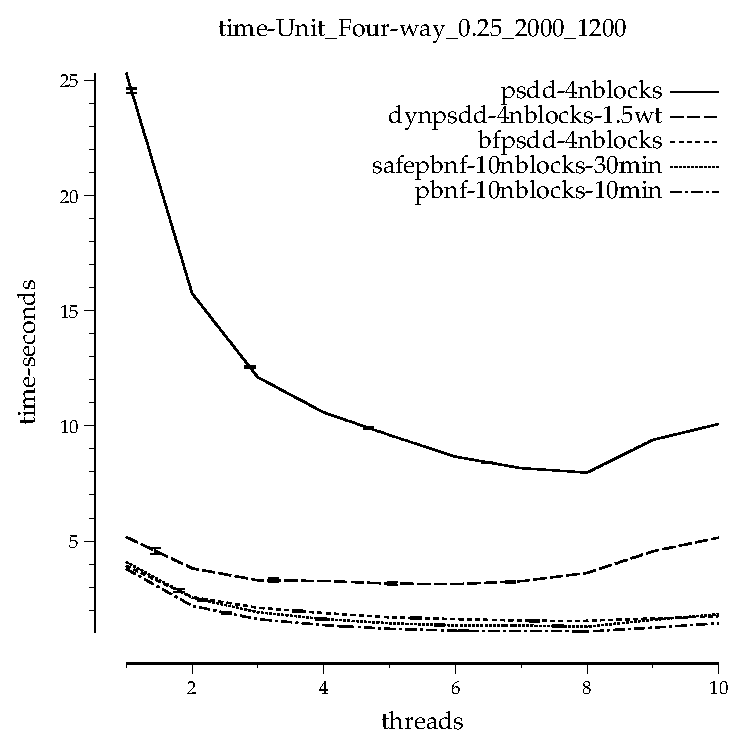
\includegraphics[width=3in]{../graphs/grid_unit_four-way_0.25_2000_1200/time-Unit_Four-way_0.25_2000_1200.eps}
\label{fig:grid-unit}
\caption{CPU time versus number of threads on a 2000x1200 unit-cost
  grid world with a 25\% probability that a square is obstructed.}
\end{figure}

\begin{figure}[t]
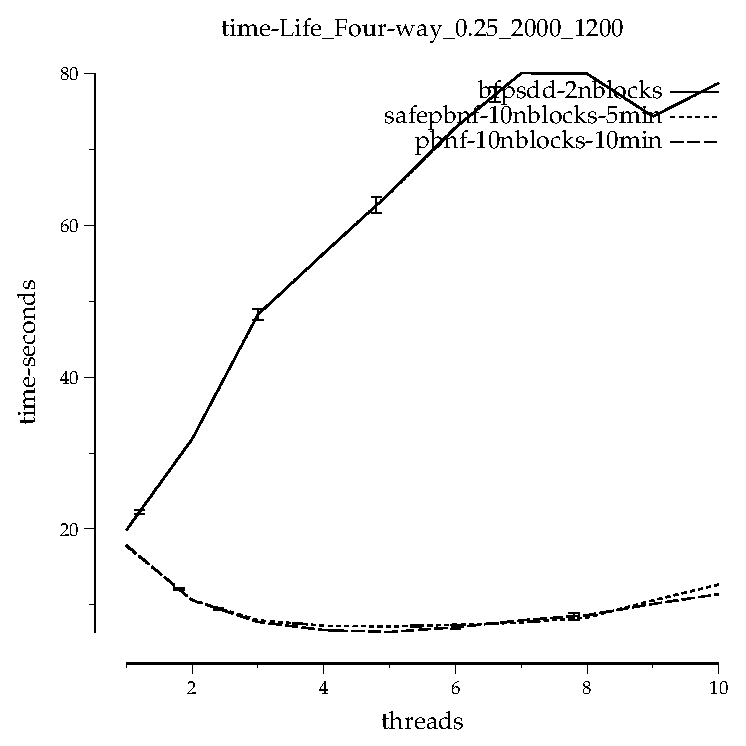
\includegraphics[width=3in]{../graphs/grid_life_four-way_0.25_2000_1200/time-Life_Four-way_0.25_2000_1200.eps}
\label{fig:grid-life}
\caption{CPU time versus number of threads on a 2000x1200 life-cost
  grid world with a 25\% probability that a square is obstructed.}
\end{figure}

\subsection{Sliding Tiles}

\section{Conclusion}
\section{Acknowledgements}

Seth, Wheeler, Rong, Jordan -- make this section better

\bibliography{master}
\bibliographystyle{aaai}

\begin{appendices}
\section{Pseudo Code}
%
% Include this file in a .tex document with \usepackage{algorithm2e}.
%

\SetKwData{block}{block}
\SetKwData{init}{init}
\SetKwData{incumbent}{incumbent}
\SetKwData{open}{open}
\SetKwData{closed}{closed}
\SetKwData{FreeList}{FreeList}
\SetKwData{minexpansions}{minexpansions}
\SetKwData{expansions}{expansions}

\SetKwFunction{threadsearch}{threadsearch}
\SetKwFunction{hot}{hot}
\SetKwFunction{interferenceScope}{interferenceScope}
\SetKwFunction{isfree}{isfree}
\SetKwFunction{setcold}{setcold}
\SetKwFunction{release}{release}
\SetKwFunction{sethot}{sethot}
\SetKwFunction{best}{best}
\SetKwFunction{shouldswitch}{shouldswitch}
\SetKwFunction{nextnblock}{nextnblock}

\begin{function*}
  \caption{search(init)}
  \KwIn{\init -- the initial node}
  \KwOut{The optimal solution, or NULL if no solution is found}
  insert \init into \open of the appropriate nblock\;
  insert \init into \closed of the appropriate nblock\;
  \lForEach{Processor}{$\threadsearch()$\;}
  \lWhile{any thread is still running}{wait\;}
  \Return incumbent
\end{function*}

\begin{function*}
  \caption{threadsearch()}
  \SetKwData{node}{node}
  \SetKwData{children}{children}
  \SetKwFunction{expand}{expand}

  \KwResult{Sets \incumbent if a solution is found}

  $\block \leftarrow$ NULL\;
  \While {{\bf not} done} {
    $\block \leftarrow \nextnblock(\block)$\;
    $\expansions \leftarrow 0$\;
    \While {{\bf not} $\shouldswitch(\block,\expansions)$} {
      $\node \leftarrow$ next node in \block\;

      \lIf {$\node > \incumbent$} {
        prune \node\;
      }

      \If {\node is a goal}{
        \lIf {$\node < \incumbent$}{
          $\incumbent \leftarrow \node$
        }
      }

      \ElseIf {\node is not a duplicate}{
        $\children \leftarrow$ \expand(\node)\;
        insert \children into \open of the appropriate nblock\;
      }

      $\expansions \leftarrow \expansions + 1$\;
    }
  }
\end{function*}

\begin{function*}
  \caption{isfree(block)}
  \KwIn{\block -- an nblock}
  \KwOut{Whether or not the given nblock is free}
  \Return $\sigma(\block) = 0$ {\bf and} $\sigma_h(\block) = 0$
          {\bf and} \block is not empty\;
\end{function*}

\begin{function*}
  \caption{shouldswitch(block, expansions)}
  \KwIn{\block -- an nblock to search,\\
    \expansions -- the number of nodes expanded in \block so far}
  \KwData{\minexpansions -- the minimum number of expansions to
    perform per-nblock}
  \KwOut{Whether or not the nblock should be switched}

  \lIf{\block is empty}{
    \Return true\;
  }
  \lIf{$\expansions < \minexpansions$}{
    \Return false\;
  }
  \If{$\best(\FreeList) < \block$ {\bf or}
    $\best(\interferenceScope(\block)) < \block$}{
    \If{$\best(\interferenceScope(\block)) < \best(\FreeList)$} {
        $\sethot(\best(\interferenceScope(\block)))$\;
    }
    \Return true\;
  }
  \ForEach{$b' \in \interferenceScope(\block)$}{
    \lIf{$\hot(b')$}{
      $\setcold(b')$\;
    }
  }
  \Return false\;
\end{function*}

\begin{function*}
  \caption{sethot(block)}
  \KwIn{\block -- an nblock}
  \KwResult{\block is flagged as hot}
  \If{{\bf not} $\hot(\block)$ {\bf and} $\sigma(\block) > 0$ {\bf
  and} $\neg\exists i \in interferenceScope(\block) : i < \block \wedge \hot(i)$ }{
    $\hot(\block) \leftarrow true$\;
    \ForEach{$n' \in \interferenceScope(\block)$}{
      \lIf{$\hot(n')$} {
        $\setcold(n')$\;
      }
      \lIf{$\isfree(n')$}{
        $\FreeList \leftarrow \FreeList \setminus \{n'\}$\;
      }
      $\sigma_h(n') \leftarrow \sigma_h(n') + 1$\;
    }
  }
\end{function*}

\begin{function*}
  \caption{setcold(block)}
  \KwIn{\block -- an nblock}
  \KwResult{\block is marked as cold}
  $\hot(\block) \leftarrow false$\;
  \ForEach{$n' \in \interferenceScope(\block)$}{
    $\sigma_h(n') \leftarrow \sigma_h(n') - 1$\;
    \If{$\isfree(n')$}{
      $\FreeList \leftarrow \FreeList \cup \{n'\}$\;
      wake all sleeping threads\;
    }
  }
\end{function*}

\begin{function*}
  \caption{release(block)}
  \KwIn{\block -- an nblock}
  \KwResult{Update the sigma values of neighboring nodes, and add them
  to the \FreeList where appropriate}
  \ForEach{$b' \in \interferenceScope(\block)$}{
    $\sigma(b') \leftarrow \sigma(b') - 1$\;
    \If{$\isfree(b')$}{
     $\FreeList \leftarrow \FreeList \cup \{b'\}$\;
     wake all sleeping threads\;
    }
  }
\end{function*}

\begin{function*}
  \caption{nextnblock(block)}
  \SetKwData{bestScope}{bestScope}
  \SetKwData{done}{done}
  \SetKwData{n}{n}

  \KwIn{\block -- an nblock}
  \KwOut{The next nblock to search}

  \lIf{\block has no open nodes}{
      lock\;
  }
  \lElseIf {trylock fails} {
          \Return \block\;
  }
  \tcc{if trylock succeeded we have the lock}

  \If{$\block \neq$ NULL}{
    $\bestScope \leftarrow \best(\interferenceScope(\block))$\;
    \If{$\block < \bestScope$ {\bf and} $\block < \best(\FreeList)$}{
      unlock\;
      \Return \block\;
    }
    \release(\block)\;
  }

  \If{$\forall b \in nblocks : \sigma(b) = 0$ {\bf and}
    \FreeList is empty} {
    $\done \leftarrow true$\;
    wake all sleeping threads\;
  }

  \lWhile{\FreeList is empty {\bf and not} \done}{
    sleep\;
  }

  \lIf{\done}{
    $\n \leftarrow$ NULL\;
  }
  \Else {
    $n \leftarrow \best(\FreeList)$\;
    \ForEach{$b' \in \interferenceScope(\n)$}{
      $\sigma(b') \leftarrow \sigma(b') + 1$\;
    }
  }

  unlock\;
  \Return $n$\;
\end{function*}


% ------------------------------------------------------------
% ------------------------------------------------------------
% ------------------------------------------------------------

\section{Plots}

The plots in this section show our experiments which were performed to
determine the best parameters for each of algorithm.

\begin{figure*}[h]
\begin{center}
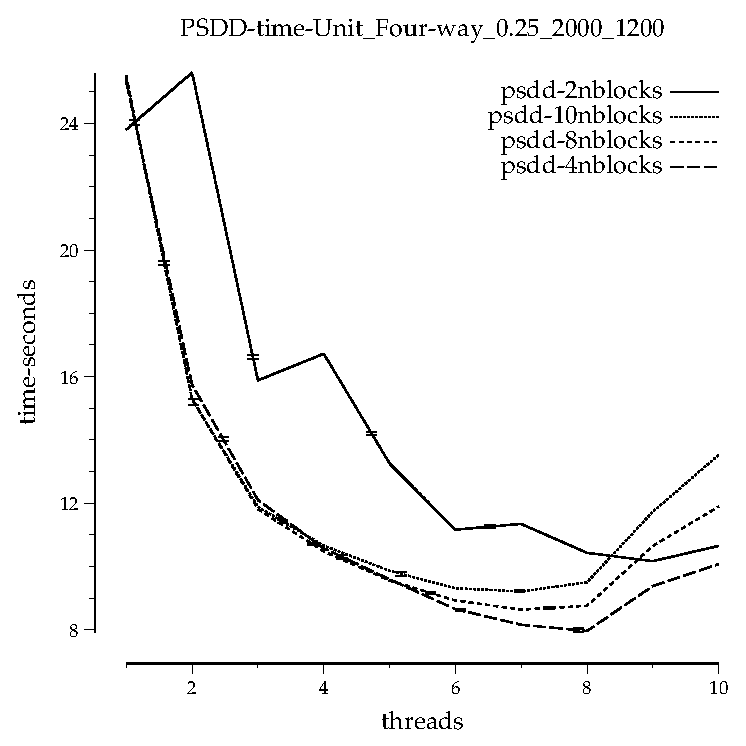
\includegraphics{../graphs/grid_unit_four-way_0.25_2000_1200/PSDD-time-Unit_Four-way_0.25_2000_1200.eps}
\caption{Wall clock time: PSDD on a 2000x1200 grid world with 25\%
  obstacles and unit cost four-way movement.}
\end{center}
\end{figure*}

\begin{figure*}[h]
\begin{center}
\includegraphics[width=3in]{../graphs/grid_unit_four-way_0.25_2000_1200/DYNPSDD-time-Unit_Four-way_0.25_2000_1200_weight=1.1.eps}
\includegraphics[width=3in]{../graphs/grid_unit_four-way_0.25_2000_1200/DYNPSDD-time-Unit_Four-way_0.25_2000_1200_weight=1.5.eps}
\includegraphics[width=3in]{../graphs/grid_unit_four-way_0.25_2000_1200/DYNPSDD-time-Unit_Four-way_0.25_2000_1200_weight=2.0.eps}
\includegraphics[width=3in]{../graphs/grid_unit_four-way_0.25_2000_1200/DYNPSDD-time-Unit_Four-way_0.25_2000_1200_weight=2.2.eps}
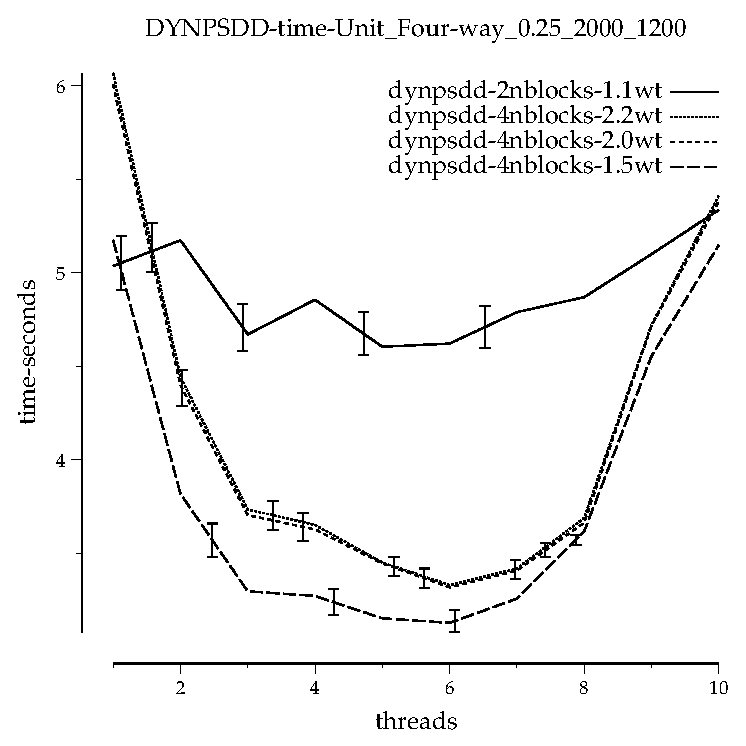
\includegraphics[width=3in]{../graphs/grid_unit_four-way_0.25_2000_1200/DYNPSDD-time-Unit_Four-way_0.25_2000_1200.eps}
\caption{Wall clock time: DYNPSDD on a 2000x1200 grid world with 25\%
  obstacles and unit cost four-way movement.  This algorithm uses wA*
  to get an upper solution cost bound, then performs PSDD using this
  bound for pruning.}
\end{center}
\end{figure*}

\begin{figure*}[h]
\begin{center}
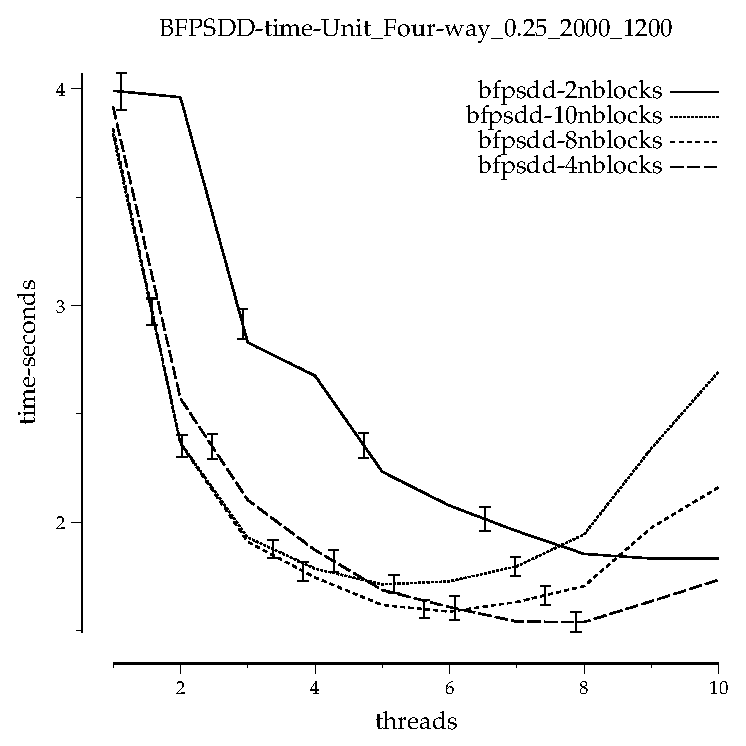
\includegraphics{../graphs/grid_unit_four-way_0.25_2000_1200/BFPSDD-time-Unit_Four-way_0.25_2000_1200.eps}
\caption{Wall clock time: Best-first PSDD on a 2000x1200 grid world with 25\%
  obstacles and unit cost four-way movement.}
\end{center}
\end{figure*}

\begin{figure*}[h]
\begin{center}
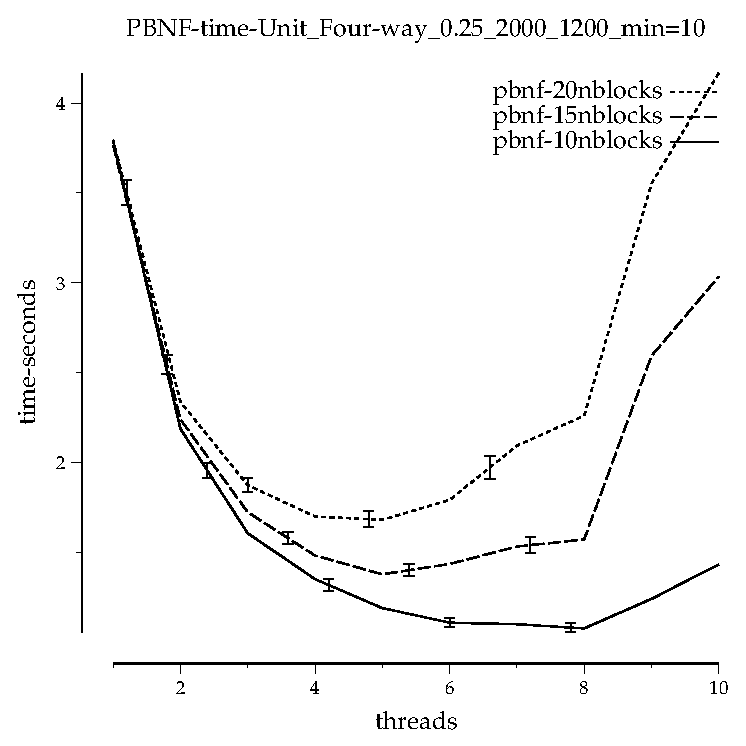
\includegraphics[width=3in]{../graphs/grid_unit_four-way_0.25_2000_1200/PBNF-time-Unit_Four-way_0.25_2000_1200_min=10.eps}
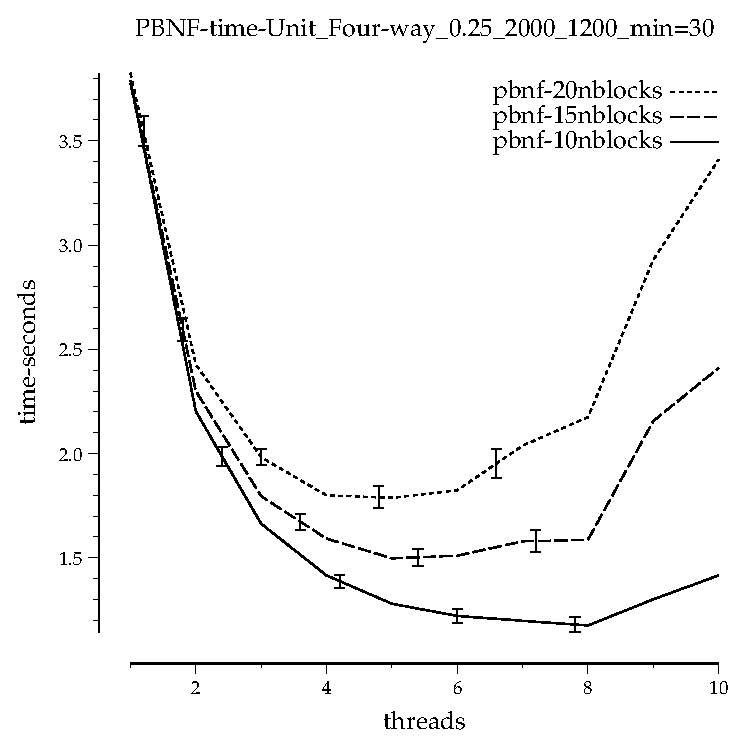
\includegraphics[width=3in]{../graphs/grid_unit_four-way_0.25_2000_1200/PBNF-time-Unit_Four-way_0.25_2000_1200_min=30.eps}
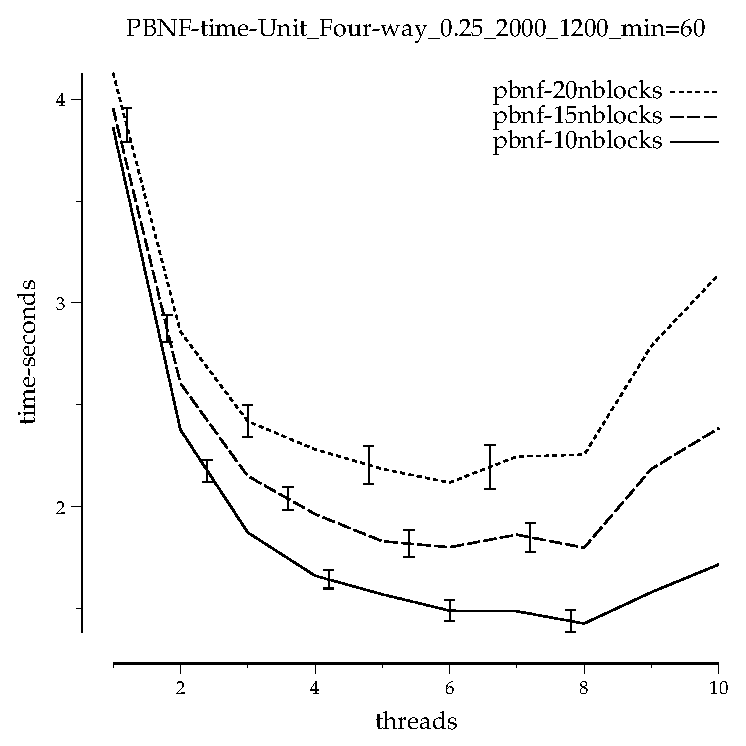
\includegraphics[width=3in]{../graphs/grid_unit_four-way_0.25_2000_1200/PBNF-time-Unit_Four-way_0.25_2000_1200_min=60.eps}
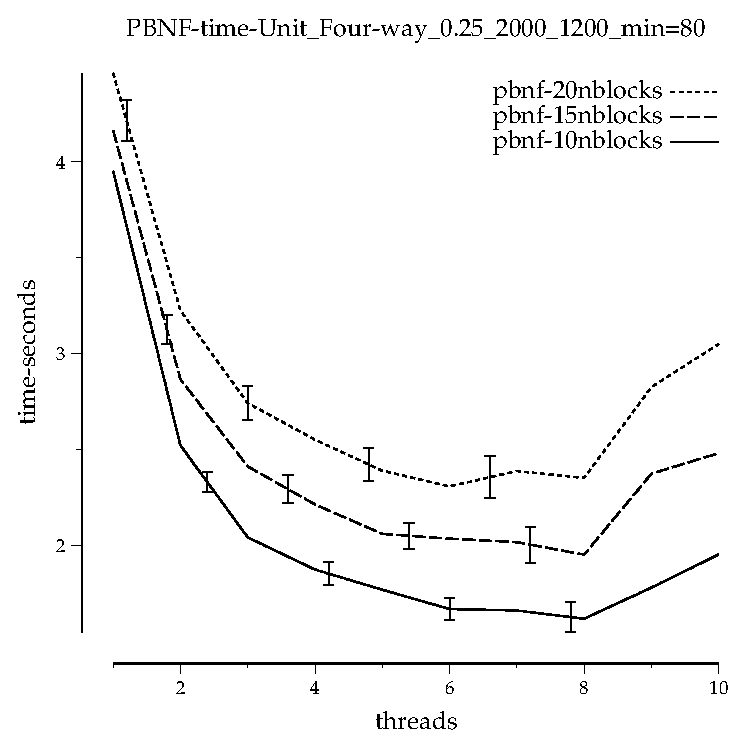
\includegraphics[width=3in]{../graphs/grid_unit_four-way_0.25_2000_1200/PBNF-time-Unit_Four-way_0.25_2000_1200_min=80.eps}
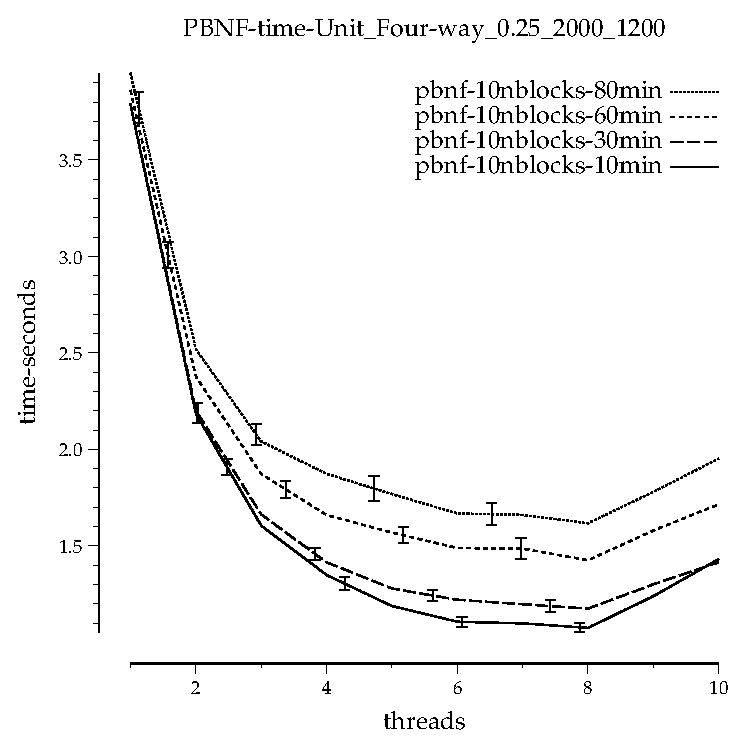
\includegraphics[width=3in]{../graphs/grid_unit_four-way_0.25_2000_1200/PBNF-time-Unit_Four-way_0.25_2000_1200.eps}
\caption{Wall clock time: PBNF on a 2000x1200 grid world with 25\%
  obstacles and unit cost four-way movement.}
\end{center}
\end{figure*}

\begin{figure*}[h]
\begin{center}
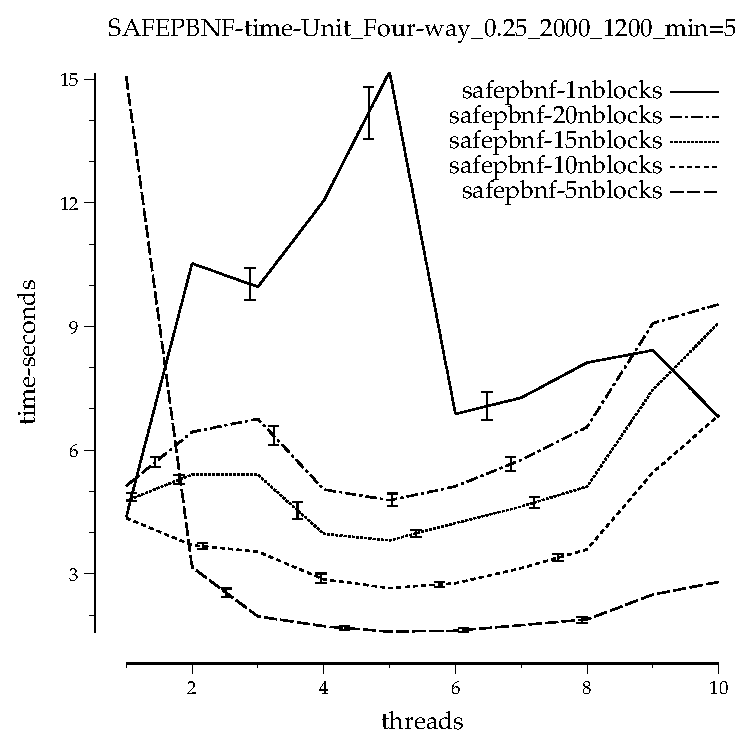
\includegraphics[width=3in]{../graphs/grid_unit_four-way_0.25_2000_1200/SAFEPBNF-time-Unit_Four-way_0.25_2000_1200_min=5.eps}
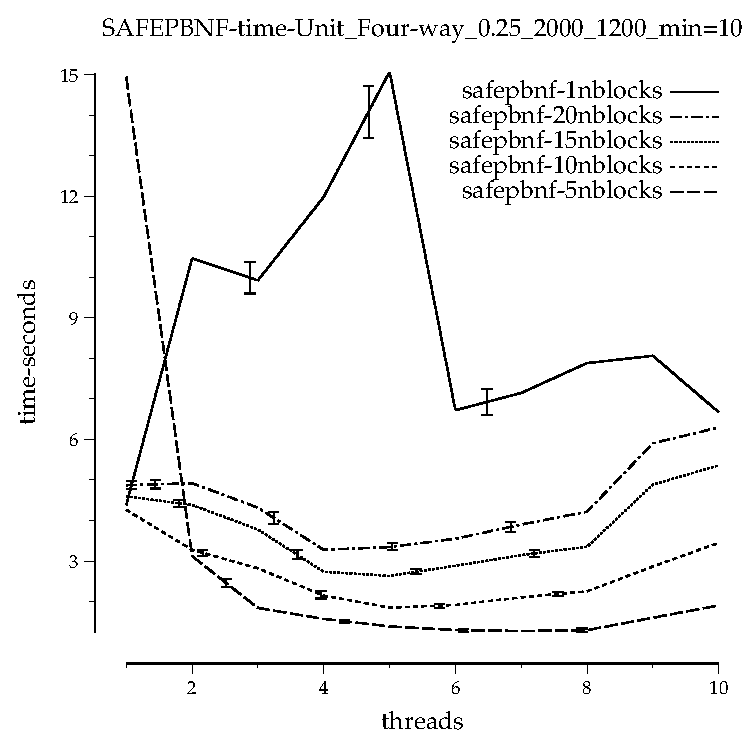
\includegraphics[width=3in]{../graphs/grid_unit_four-way_0.25_2000_1200/SAFEPBNF-time-Unit_Four-way_0.25_2000_1200_min=10.eps}
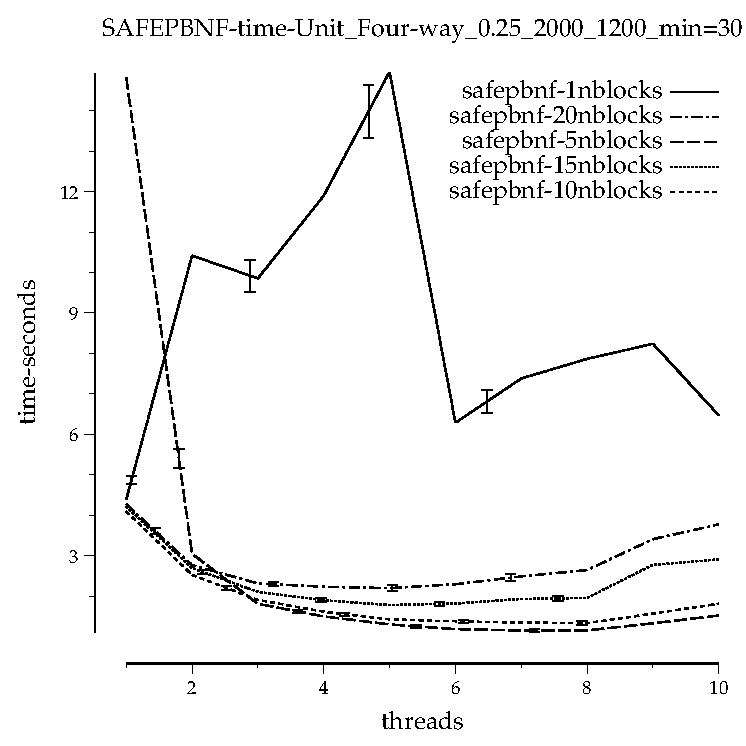
\includegraphics[width=3in]{../graphs/grid_unit_four-way_0.25_2000_1200/SAFEPBNF-time-Unit_Four-way_0.25_2000_1200_min=30.eps}
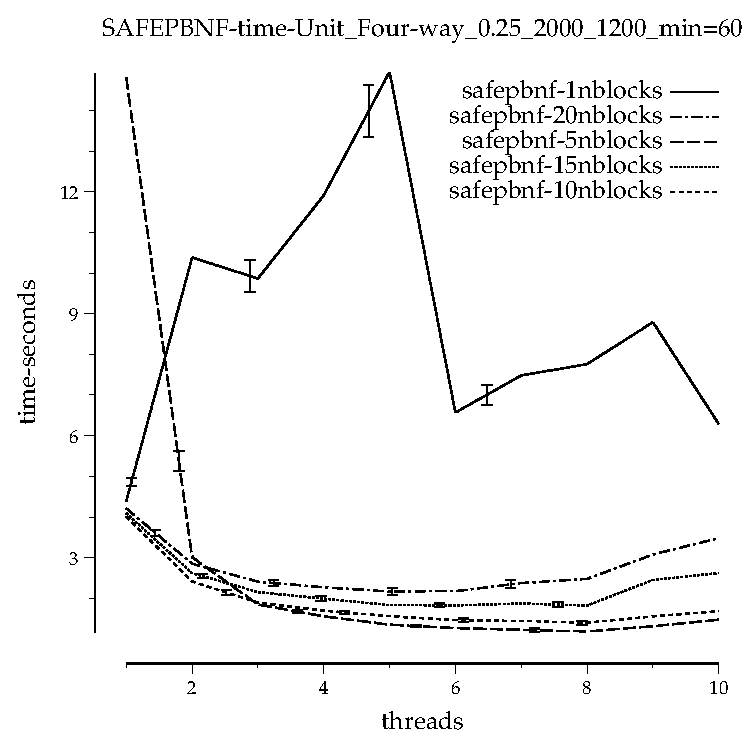
\includegraphics[width=3in]{../graphs/grid_unit_four-way_0.25_2000_1200/SAFEPBNF-time-Unit_Four-way_0.25_2000_1200_min=60.eps}
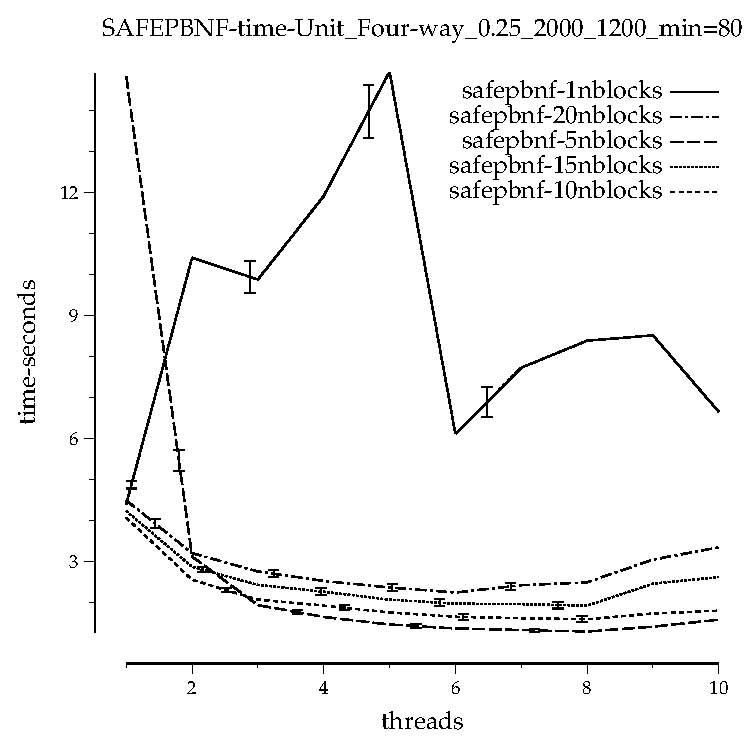
\includegraphics[width=3in]{../graphs/grid_unit_four-way_0.25_2000_1200/SAFEPBNF-time-Unit_Four-way_0.25_2000_1200_min=80.eps}
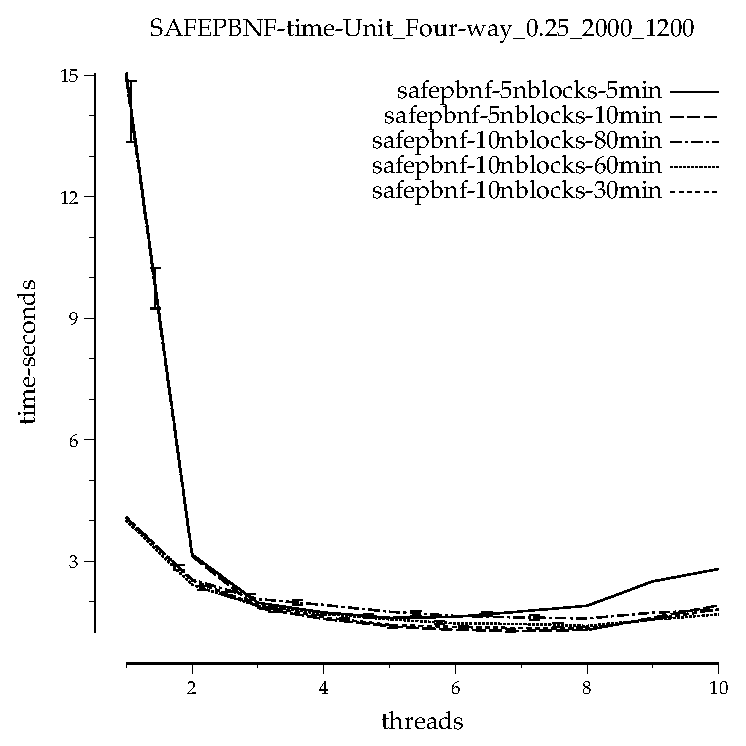
\includegraphics[width=3in]{../graphs/grid_unit_four-way_0.25_2000_1200/SAFEPBNF-time-Unit_Four-way_0.25_2000_1200.eps}
\caption{Wall clock time: Safe PBNF on a 2000x1200 grid world with 25\%
  obstacles and unit cost four-way movement.}
\end{center}
\end{figure*}

% ------------------------------------------------------------

\begin{figure*}[h]
\begin{center}
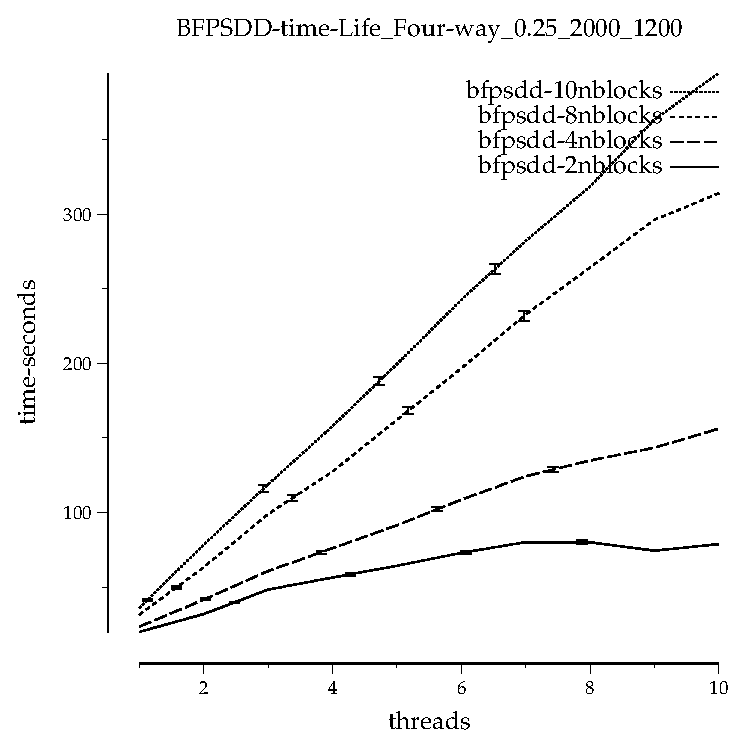
\includegraphics{../graphs/grid_life_four-way_0.25_2000_1200/BFPSDD-time-Life_Four-way_0.25_2000_1200.eps}
\caption{Wall clock time: Best-first PSDD on a 2000x1200 grid world with 25\%
  obstacles and life cost four-way movement.}
\end{center}
\end{figure*}

\begin{figure*}[h]
\begin{center}
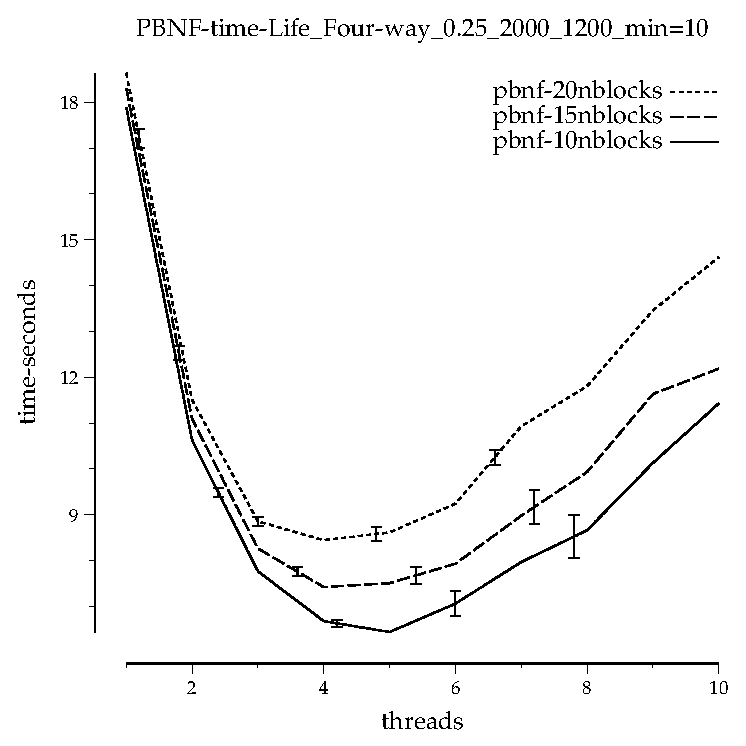
\includegraphics[width=3in]{../graphs/grid_life_four-way_0.25_2000_1200/PBNF-time-Life_Four-way_0.25_2000_1200_min=10.eps}
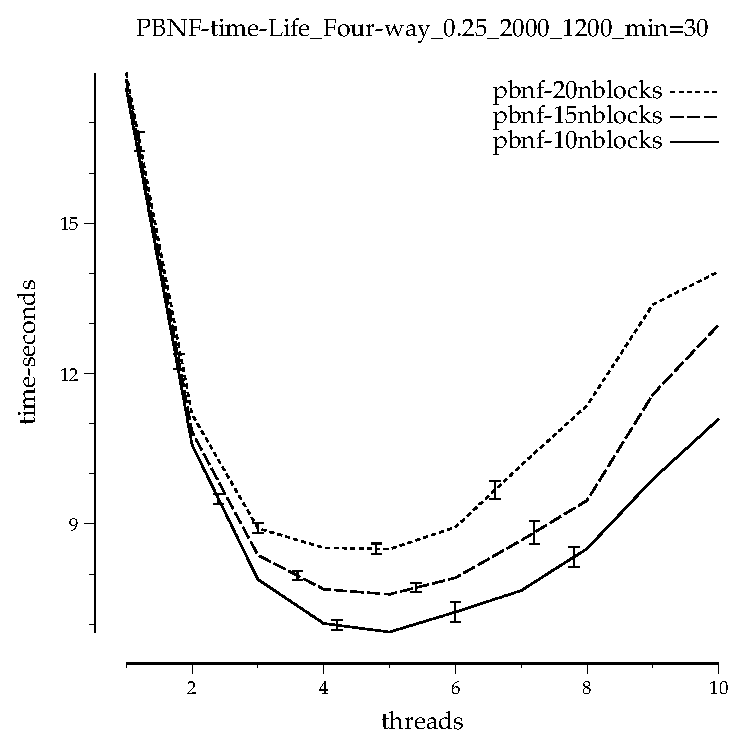
\includegraphics[width=3in]{../graphs/grid_life_four-way_0.25_2000_1200/PBNF-time-Life_Four-way_0.25_2000_1200_min=30.eps}
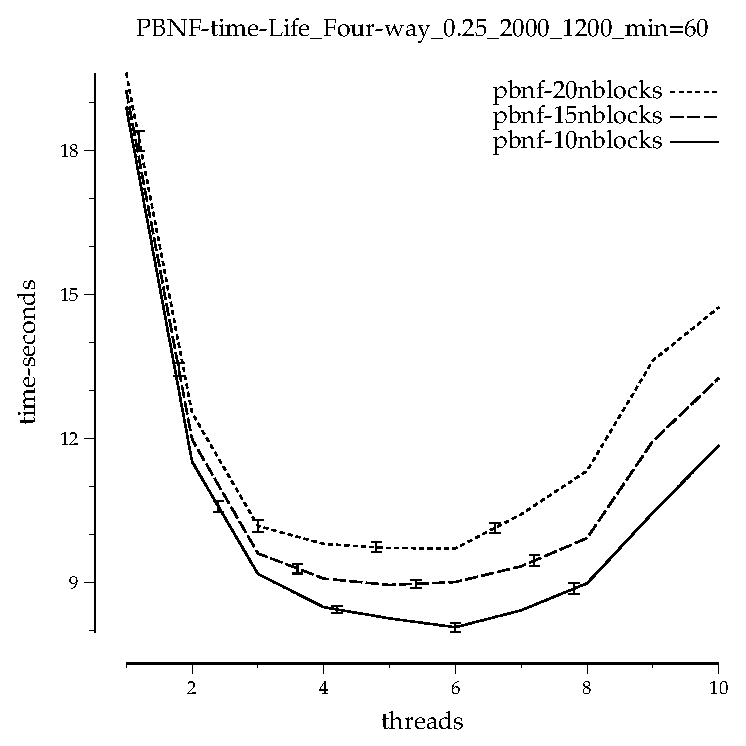
\includegraphics[width=3in]{../graphs/grid_life_four-way_0.25_2000_1200/PBNF-time-Life_Four-way_0.25_2000_1200_min=60.eps}
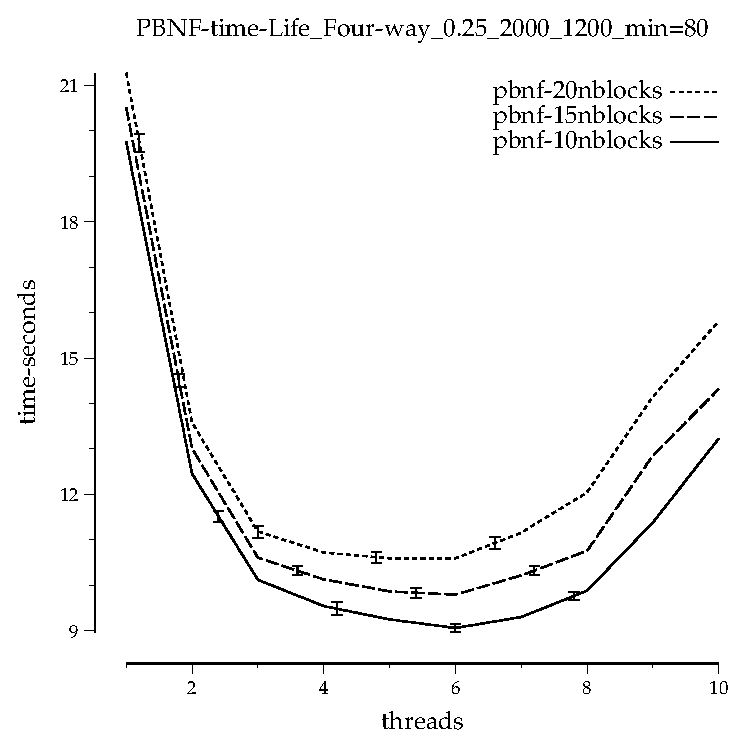
\includegraphics[width=3in]{../graphs/grid_life_four-way_0.25_2000_1200/PBNF-time-Life_Four-way_0.25_2000_1200_min=80.eps}
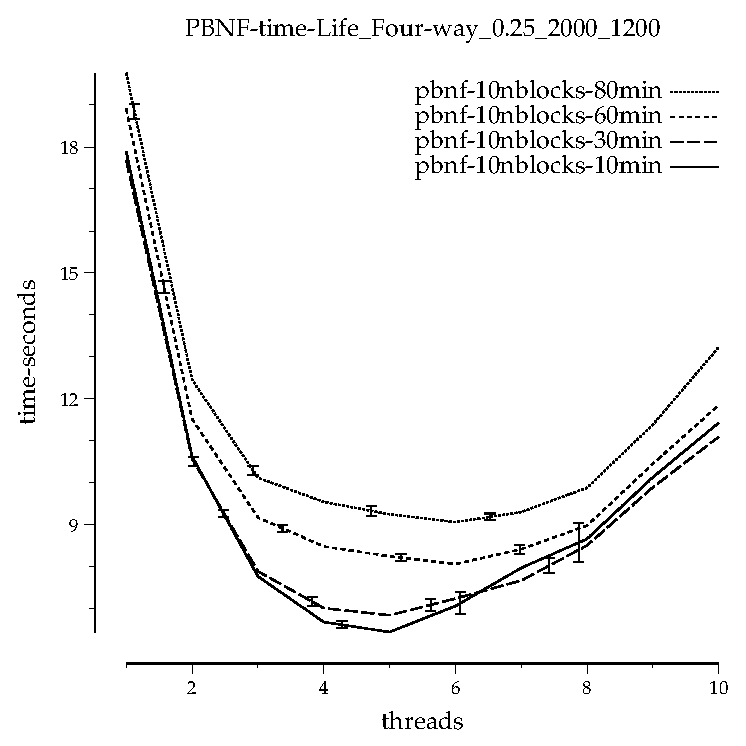
\includegraphics[width=3in]{../graphs/grid_life_four-way_0.25_2000_1200/PBNF-time-Life_Four-way_0.25_2000_1200.eps}
\caption{Wall clock time: PBNF on a 2000x1200 grid world with 25\%
  obstacles and life cost four-way movement.}
\end{center}
\end{figure*}

\begin{figure*}[h]
\begin{center}
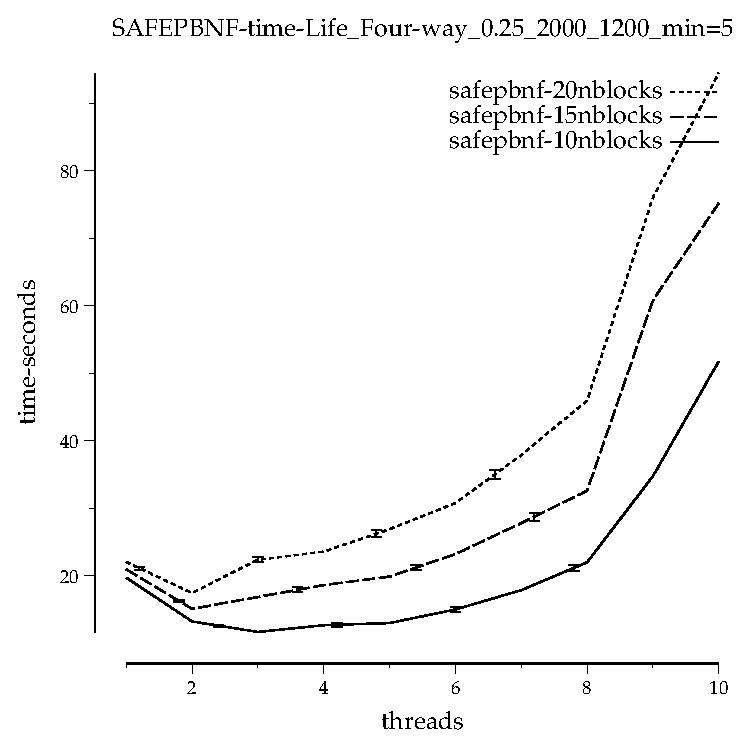
\includegraphics[width=3in]{../graphs/grid_life_four-way_0.25_2000_1200/SAFEPBNF-time-Life_Four-way_0.25_2000_1200_min=5.eps}
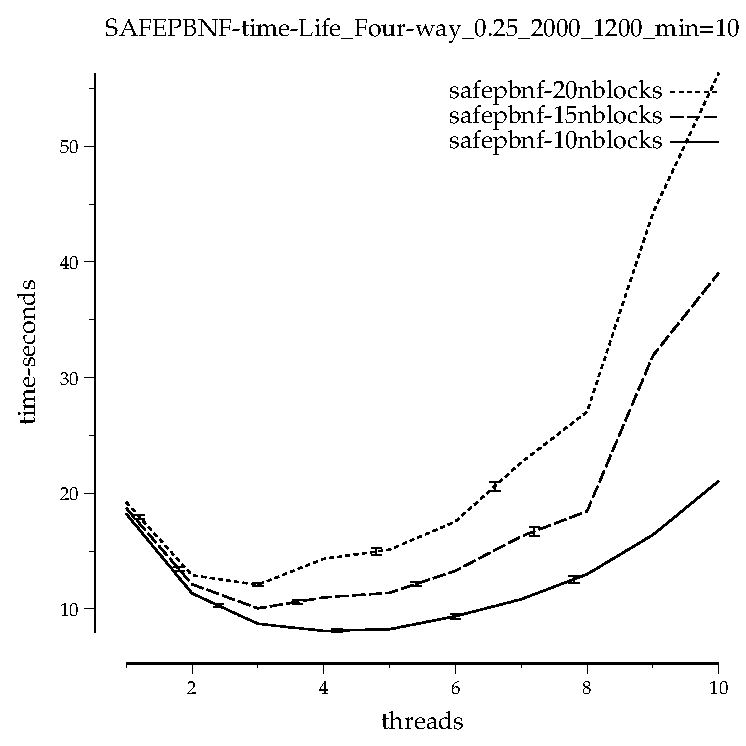
\includegraphics[width=3in]{../graphs/grid_life_four-way_0.25_2000_1200/SAFEPBNF-time-Life_Four-way_0.25_2000_1200_min=10.eps}
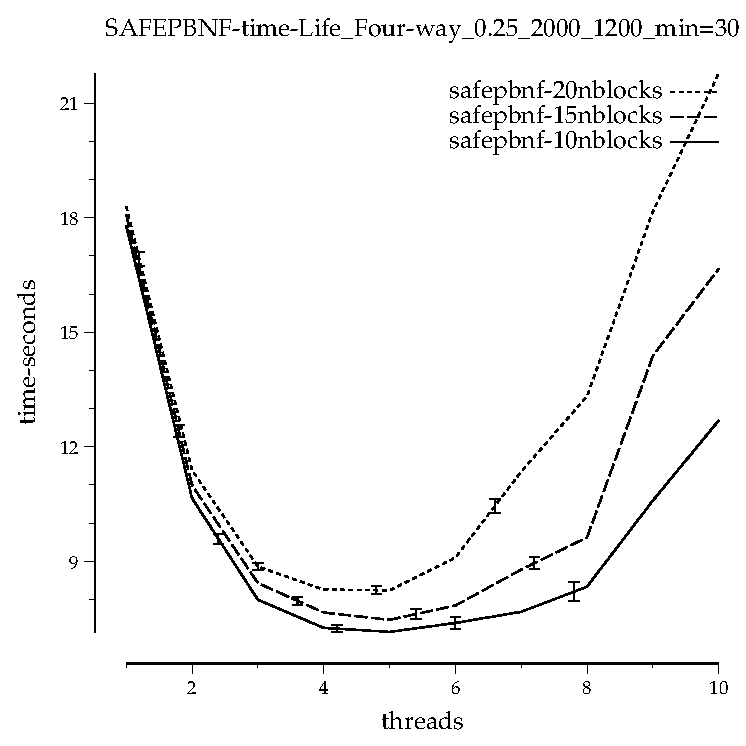
\includegraphics[width=3in]{../graphs/grid_life_four-way_0.25_2000_1200/SAFEPBNF-time-Life_Four-way_0.25_2000_1200_min=30.eps}
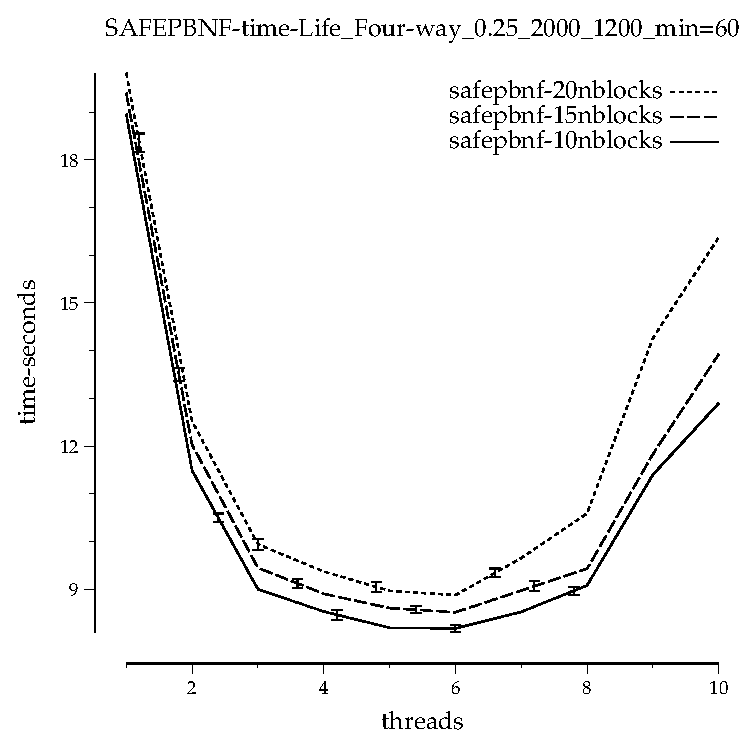
\includegraphics[width=3in]{../graphs/grid_life_four-way_0.25_2000_1200/SAFEPBNF-time-Life_Four-way_0.25_2000_1200_min=60.eps}
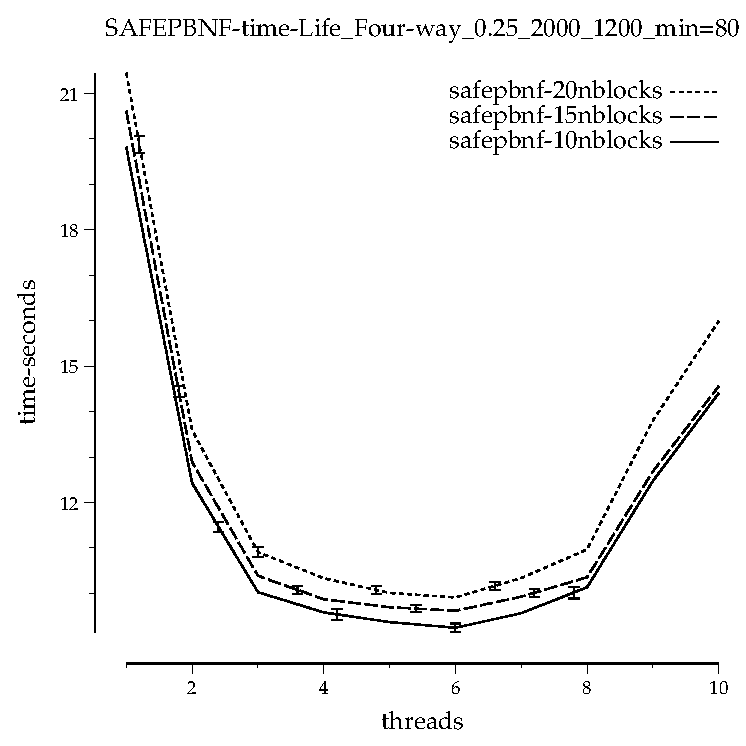
\includegraphics[width=3in]{../graphs/grid_life_four-way_0.25_2000_1200/SAFEPBNF-time-Life_Four-way_0.25_2000_1200_min=80.eps}
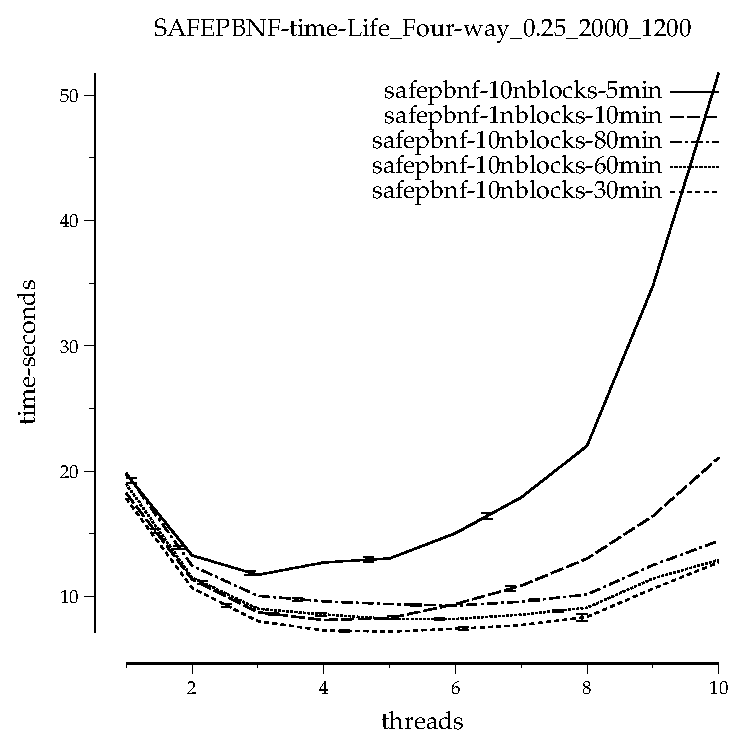
\includegraphics[width=3in]{../graphs/grid_life_four-way_0.25_2000_1200/SAFEPBNF-time-Life_Four-way_0.25_2000_1200.eps}
\caption{Wall clock time: Safe PBNF on a 2000x1200 grid world with 25\%
  obstacles and life cost four-way movement.}
\end{center}
\end{figure*}

% ------------------------------------------------------------
% ------------------------------------------------------------
% ------------------------------------------------------------

\end{appendices}

\end{document}
